\section{Experiments}
\label{sec:experiments}

\begin{figure*}[t]
\centering
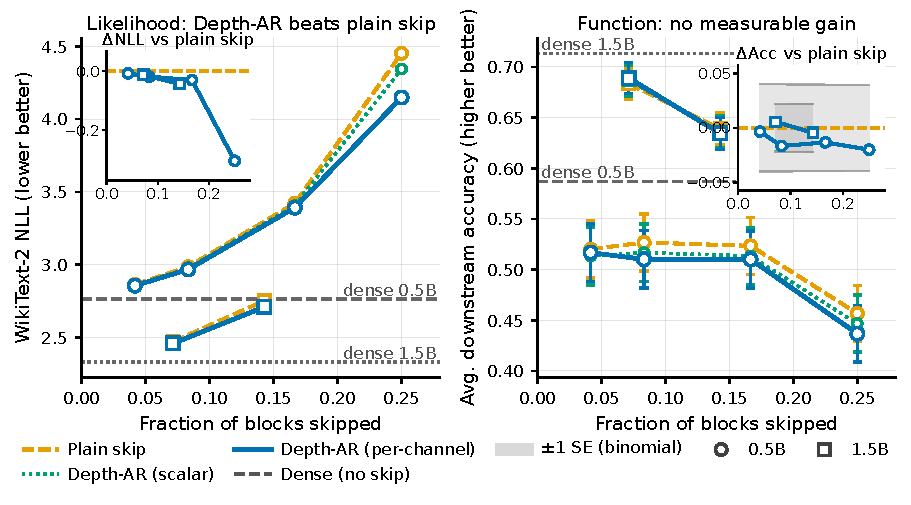
\includegraphics[width=0.62\textwidth]{figures/fig2_dissociation.pdf}
\caption{\textbf{Prediction pays off in proportion to what skipping destroys.} Quality against
the fraction of blocks skipped for Qwen2.5-0.5B (circles), 1.5B (squares) and 7B (triangles),
layers chosen by measured residual damage, the deployable rule, with every predictor skipping
the identical blocks. Bands are binomial standard error with the measured 0.44-point
harness jitter folded in quadrature (\Cref{sec:app-noise}); the lighter outer band is
$1.96$~SE. Where skipping barely hurts, at the left of each panel, \mname and plain skipping
are indistinguishable in behaviour, and the differences there lie below the evaluation's own
reproducibility floor. Where skipping does severe damage the gap opens: at 28.6\% of
blocks skipped on 7B, \mname answers 89 more questions correctly out of 900 than
plain skipping ($z=4.31$, surviving Bonferroni correction across all 63
comparisons) while recovering 38.1\% of its language-modelling damage. Both breakdowns
are drawn rather than hidden: at 42.9\% skipped on 7B the depth-only predictor falls
\emph{below} plain skipping on likelihood, where the cross-token extension of
\Cref{sec:app-crosstoken} does not. Hardware and protocol: \Cref{sec:app-protocol}.}
\label{fig:dissociation}
\end{figure*}


\paragraph{Setup.} We evaluate Qwen2.5-0.5B, Qwen2.5-1.5B and Qwen2.5-\topscale
\citep{qwen2025}. Coefficients are fitted in closed form (\cref{eq:fit}) on unlabeled
WikiText-103 \citep{merity2017pointer} and scored on a disjoint held-out split; no task
data is used for calibration. We report NLL and accuracy on HellaSwag
\citep{zellers2019hellaswag}, PIQA \citep{bisk2020piqa} and ARC-Easy
\citep{clark2018think} (100 examples per task on 0.5B, 300 on 1.5B and
\topscale), and give accuracy deltas as absolute counts, since recovered-gap fractions
divide by very small denominators. Skipped blocks are non-adjacent, and within a budget
every predictor skips the \emph{identical} blocks, isolating the predictor from the
selection rule. Full protocol, hardware and precisions in \Cref{sec:app-protocol}. Every accuracy effect we
report is measured against three quantified sources of uncertainty: the binomial standard error
of the difference, Bonferroni correction across the full family of 63 comparisons we run,
and the evaluation harness's own measured batch-shape jitter (\Cref{sec:app-noise}). One
prediction in this paper was pre-registered before its data existed, and we report its outcome
either way (\Cref{sec:app-crosstoken}).

\paragraph{A single coefficient per layer is not enough.} \Cref{tab:selection} (\Cref{sec:app-selection}) reports the
fraction of plain-skip NLL damage each predictor recovers under three rules for choosing
which blocks to skip. The scalar predictor of \cref{eq:ar1} is not a mildly weaker \mname:
under the cheap rule it is \emph{worse} than plain skipping, recovering $-0.745$ of
the damage at $k=2$. One coefficient per channel, nothing else changed, turns that into
$+0.053$. \mname recovers more damage than every alternative under \emph{every} rule
and both budgets, so it composes with whichever selection method a practitioner already
uses. Copy Update is worse than plain skipping everywhere, so the benefit comes from
\emph{fitting} the coefficients, not from injecting a nonzero update.

\paragraph{At a matched budget, likelihood recovery grows with scale.} \Cref{tab:main} carries
the comparison to downstream tasks: at the light, damage-based operating point \mname recovers
4.6\%, 10.3\% and 23.3\% of the plain-skip damage on 0.5B, 1.5B and 7B at $k=4$. The trend is
budget-specific: at $k=2$ recovery is flat to mildly declining with scale (8.4\%, 8.2\%,
7.3\%), so we claim no general scaling law. The scalar predictor recovers consistently less, and Copy Update is
worse than not predicting at all.

\paragraph{The downstream benefit scales with the damage skipping inflicts.} Accuracy is
where the skip operator either matters or does not, and what decides which is not the
selection rule but how much damage skipping does. At light budgets, where plain skipping
barely hurts, no accuracy difference is significant at any scale (largest $z=1.18$),
and the differences are smaller than the evaluation's own reproducibility floor. Where the
damage is severe, the gains are large. Under the \emph{deployable} damage-based rule at
28.6\% of blocks skipped on Qwen2.5-7B, \mname answers 89 more questions
correctly out of 900 than plain skipping ($z=4.31$), recovering 38.1\% of
the language-modelling damage and 35.7\% of the accuracy gap. Under damage-seeking
selection on Qwen2.5-1.5B it answers 132 and 90 more ($z=6.45$,
$4.37$). These are 4 of 63 comparisons and the only ones to survive
Bonferroni correction. Prediction pays off in proportion to what skipping destroys.

These are gains over a badly damaged baseline (61.7\% average accuracy against a dense 79.4\%),
not a claim that the compressed model matches dense quality, and the pattern has a limit
(\Cref{sec:app-pareto}).

\paragraph{Predictability does not imply recoverability.} Held-out predictability $P_\ell$ and
the damage a predictor actually repairs are statistically unrelated (Spearman $-0.015$,
$p=0.95$; \Cref{fig:momentum}), and choosing layers by $P_\ell$ is not merely suboptimal but
actively harmful. Accurate reconstruction in residual space is not the same objective as
preserving function, and the same blindness recurs when an energy-weighted criterion tunes the
predictor itself (\Cref{sec:app-ridge}).

\paragraph{The forecast is cheap, and it buys frontier position.} On Qwen2.5-7B at four
skipped blocks, \mname adds 0.64\% \emph{prefill} latency over plain skipping at
sequence length 512, retaining a 1.141$\times$ prefill speedup over the dense model
(1.151$\times$ at 2048) where plain skipping reaches 1.148$\times$
(\Cref{sec:app-latency}). The two methods sit at effectively the same point on the compute
axis, so all of \mname's advantage is quality at that point (\Cref{sec:app-pareto}). We measure
prefill latency at $k=4$ only and make no claim about end-to-end generation.

The practical guidance follows. At light budgets plain skipping leaves little repairable damage
behind, and \mname improves likelihood but buys no measurable behaviour. Under aggressive
pruning, where skipping is destructive enough to be worth repairing, it recovers large and
statistically significant quality for roughly half a percent of prefill latency. Repair the
update when skipping is expensive; do not bother when it is cheap.

\paragraph{Limitations.}
\label{sec:limitations}
At \emph{light} budgets, where plain skipping already preserves most of the model,
the likelihood \mname recovers does not register as a downstream accuracy gain. At $k \le 4$ no
accuracy difference is significant at any of the three scales, and those differences are smaller
than the run-to-run variation of the evaluation itself (\Cref{sec:app-noise}). We claim no
downstream improvement at those light budgets, and symmetrically no harm. Our evidence is also drawn from one model family. Running the deployable configuration on
Qwen3 (0.6B to 8B) under the same protocol, recovery is non-monotone in model size and absent at
1.7B despite that being the most damaged cell, so neither the scale trend nor the damage ordering
should be read as universal; the cross-token extension's advantage, by contrast, does replicate
there (\Cref{sec:app-qwen3}). Translating light-budget likelihood
recovery into accuracy, and understanding that exception, are the natural next steps. We also leave open \emph{why} the per-channel predictor succeeds
where the scalar fails (\Cref{sec:app-experiments}). One clue: a \textbf{cross-token}
variant, which also reads the previous \emph{token}'s update from the preceding layer, turns
layer 2, the one pathology no ridge could suppress, from a recovery of $-3.31$ into
$+0.19$, so that failure was missing information, not mis-regularisation. It does not
improve \mname at deployable layer sets; we report it as preliminary in
\Cref{sec:app-crosstoken}.
